\documentclass[aspectratio=169,11pt]{beamer}
\usetheme{Madrid}
\usecolortheme{seahorse}
\setbeamertemplate{navigation symbols}{}
\usepackage[T1]{fontenc}
\usepackage{lmodern}
\usepackage{booktabs}
\usepackage{array}
\usepackage{xcolor}
\usepackage{listings}
\usepackage{amsmath}
\usepackage{amssymb}
\usepackage{tikz}
\usetikzlibrary{arrows.meta,positioning,calc,decorations.pathreplacing,fit}

\newcommand{\code}[1]{\texttt{\detokenize{#1}}}
\newcommand{\NaN}{NaN}
\definecolor{nanred}{RGB}{214,39,40}
\definecolor{validblue}{RGB}{31,119,180}
\definecolor{padgray}{RGB}{150,150,150}
\definecolor{maskdark}{RGB}{60,60,60}
\definecolor{infor}{RGB}{255,127,14}
\definecolor{okgreen}{RGB}{44,160,44}
\lstset{basicstyle=\ttfamily\scriptsize, columns=fullflexible, keepspaces=true, breaklines=true,
        backgroundcolor=\color{black!4}, frame=single, rulecolor=\color{black!15}, language=C++,
        showstringspaces=false, escapeinside={(*@}{@*)}}
\tikzset{
  op/.style={draw, rounded corners=2pt, fill=white, minimum height=7mm, align=center, font=\scriptsize, inner sep=2pt},
  mat/.style={draw, fill=validblue!12, align=center, font=\scriptsize, inner sep=1pt},
  hbm/.style={draw, fill=nanred!10, align=center, font=\scriptsize, inner sep=2pt},
  arr/.style={-{Stealth[length=2mm]}, thick, black!65},
}
\newcommand{\legendbox}[1]{\tikz[baseline=-0.6ex]\node[draw=black!40, fill=#1, minimum width=2.6mm, minimum height=2.6mm, inner sep=0pt]{};}

\title[Flash attention, tile by tile]{Flash Attention, Tile by Tile}
\subtitle{From a plain attention block to PyTorch's flash kernels: padding lanes, stale shared memory,\\ and when \texttt{lse\_sum != lse\_sum} fires}
\author[SC26 nixnan tutorial]{SC26 nixnan tutorial}
\institute[]{\texttt{flash-attn-expt}, branch \texttt{Flash-Attn}}
\date{October 2026}

\begin{document}

\begin{frame}
\titlepage
\end{frame}

%-----------------------------------------------------------------------------
\begin{frame}{Roadmap}
\begin{enumerate}
\item \textbf{A plain attention block}: $O = \mathrm{softmax}(\sigma QK^\top + \text{mask})\,V$, and why it is memory-bound
\item \textbf{Massaging it into flash attention}: online softmax, tiles, one fused kernel; the split-KV variant and its combine kernel
\item \textbf{Padding lanes}: a decode step that fills one row of a $128\times128$ tile; the unloaded rows hold the \emph{previous launch's} \NaN-laden output
\item \textbf{How flash computes on them, and why discarding is safe}
\item \textbf{The combine guard \code{lse_sum != lse_sum}}: scenarios where it does \emph{not} fire, and a proof that it cannot for any positive scale
\item \textbf{Making it fire}: a negative softmax scale
\end{enumerate}
\vspace{2mm}
\small All numbers come from PyTorch 2.6's own flash source, rebuilt with dump hooks and verified \textbf{bitwise-equal} to PyTorch's kernel, running TinyGPT (4 layers, 4 heads, head dim 32) on an RTX 3090.
\end{frame}

%=============================================================================
\section{Plain attention}

\begin{frame}{Attention in one line}
\begin{columns}[T]
\begin{column}{0.52\textwidth}
For one head, with $N$ queries, $N_k$ keys and head dimension $d$:
\[
S = \sigma\, Q K^\top \in \mathbb{R}^{N\times N_k},\qquad \sigma = \tfrac{1}{\sqrt d}
\]
\[
P_{ij} = \frac{e^{S_{ij}}}{\sum_{j'} e^{S_{ij'}}},\qquad O = P\,V \in \mathbb{R}^{N\times d}
\]
\begin{itemize}\small
\item Row $i$ of $O$ is a weighted average of the rows of $V$; the weights come from how well query $i$ matches each key
\item \textbf{Causal mask}: $S_{ij}=-\infty$ for $j>i$, so $P_{ij}=0$
\item \textbf{Rows are independent}: row $i$ of $O$ needs only row $i$ of $Q$ (and all of $K$, $V$)
\end{itemize}
\end{column}
\begin{column}{0.46\textwidth}
\begin{block}{TinyGPT's attention}\small
4 heads, $d=32$, $\sigma=1/\sqrt{32}\approx0.177$\\
Q, K, V in FP16 (\code{q.half()} etc.)\\
\code{F.scaled_dot_product_attention} with the flash backend forced (as HF models such as BioMistral do)
\end{block}
\begin{block}{Two kinds of calls}\small
\textbf{training / prefill}: $N=N_k=T$, causal\\
\textbf{decode} (KV cache): $N=1$ new query, $N_k$ = all keys so far, no mask needed
\end{block}
\end{column}
\end{columns}
\end{frame}

%-----------------------------------------------------------------------------
\begin{frame}{A plain attention block}
\centering
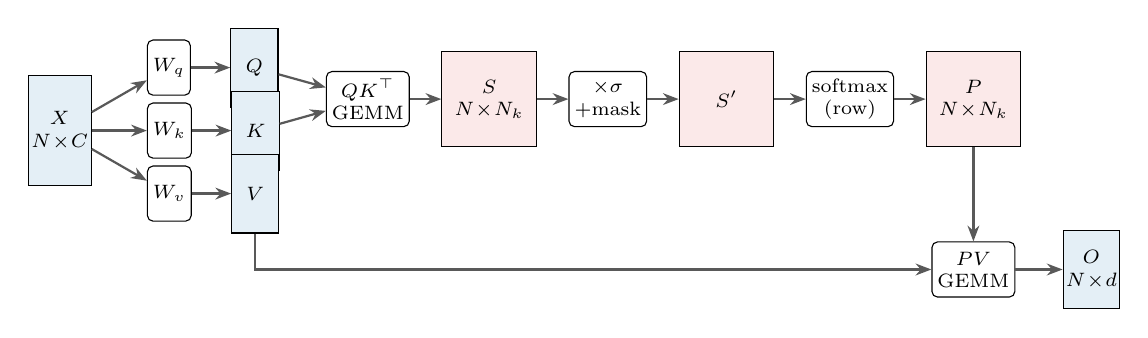
\begin{tikzpicture}[node distance=4mm]
\node[mat, minimum width=8mm, minimum height=14mm] (x) {$X$\\$N\!\times\!C$};
\node[op, right=7mm of x, yshift=8mm] (wq) {$W_q$};
\node[op, right=7mm of x] (wk) {$W_k$};
\node[op, right=7mm of x, yshift=-8mm] (wv) {$W_v$};
\node[mat, right=5mm of wq, minimum width=6mm, minimum height=10mm] (q) {$Q$};
\node[mat, right=5mm of wk, minimum width=6mm, minimum height=10mm] (k) {$K$};
\node[mat, right=5mm of wv, minimum width=6mm, minimum height=10mm] (v) {$V$};
\node[op, right=6mm of q, yshift=-4mm] (mm1) {$QK^\top$\\GEMM};
\node[hbm, right=4mm of mm1, minimum width=12mm, minimum height=12mm] (s) {$S$\\$N\!\times\!N_k$};
\node[op, right=4mm of s] (sc) {$\times\sigma$\\$+$mask};
\node[hbm, right=4mm of sc, minimum width=12mm, minimum height=12mm] (s2) {$S'$};
\node[op, right=4mm of s2] (sm) {softmax\\(row)};
\node[hbm, right=4mm of sm, minimum width=12mm, minimum height=12mm] (p) {$P$\\$N\!\times\!N_k$};
\node[op, below=12mm of p] (mm2) {$PV$\\GEMM};
\node[mat, right=6mm of mm2, minimum width=6mm, minimum height=10mm] (o) {$O$\\$N\!\times\!d$};
\draw[arr] (x) -- (wq); \draw[arr] (x) -- (wk); \draw[arr] (x) -- (wv);
\draw[arr] (wq) -- (q); \draw[arr] (wk) -- (k); \draw[arr] (wv) -- (v);
\draw[arr] (q) -- (mm1); \draw[arr] (k) -- (mm1);
\draw[arr] (mm1) -- (s); \draw[arr] (s) -- (sc); \draw[arr] (sc) -- (s2); \draw[arr] (s2) -- (sm); \draw[arr] (sm) -- (p);
\draw[arr] (p) -- (mm2); \draw[arr] (v.south) |- (mm2.west); \draw[arr] (mm2) -- (o);
\end{tikzpicture}
\vspace{3mm}
\begin{itemize}\small
\item Written this way, every step is a separate kernel, and \textcolor{nanred}{$S$, $S'$ and $P$ are $N\times N_k$ matrices written to and read from GPU memory (HBM)}
\item For $N=N_k=4096$, one head: 16M entries per matrix, versus 128K for $Q$ ($d=32$)
\item The arithmetic is cheap; \textbf{the traffic dominates}. Attention is memory-bound and quadratic in memory
\end{itemize}
\end{frame}

%-----------------------------------------------------------------------------
\begin{frame}{Softmax in practice: max subtraction and the log-sum-exp}
\begin{columns}[T]
\begin{column}{0.53\textwidth}
\begin{itemize}\small
\item $e^{S}$ overflows FP32 for $S>88.7$, so every implementation subtracts the row max $m_i=\max_j S_{ij}$:
\[
P_{ij} = \frac{e^{S_{ij}-m_i}}{\ell_i},\qquad \ell_i = \sum_j e^{S_{ij}-m_i}
\]
\item Every exponent is $\le 0$; the maximal term is exactly $e^0=1$, so $\ell_i\in[1,N_k]$
\item The \textbf{log-sum-exp} summarizes a row:
\[
\mathrm{lse}_i = \log\sum_j e^{S_{ij}} = m_i + \log \ell_i
\]
\item With it, $P_{ij}=e^{S_{ij}-\mathrm{lse}_i}$. Flash stores it for the backward pass and to merge partial results
\end{itemize}
\end{column}
\begin{column}{0.45\textwidth}
\begin{block}{Two edge cases a kernel must handle}\small
\textbf{fully masked row}: every $S_{ij}=-\infty$, $m_i=-\infty$, $e^{-\infty-(-\infty)}=$ \NaN{}. Kernels special-case $m=-\infty$.\\[2mm]
\textbf{\NaN{} anywhere in the row}: $\ell_i=$ \NaN{}.\\[2mm]
Flash's \code{softmax.h} guards both: if $\ell=0$ or $\ell\neq\ell$, it sets the LSE to $\pm\infty$ instead of $m+\log\ell$.
\end{block}
\end{column}
\end{columns}
\end{frame}

%=============================================================================
\section{From plain to flash}

\begin{frame}{The flash idea: never materialize $S$ and $P$}
\begin{enumerate}
\item \textbf{Tile}: cut $Q$ into row blocks $Q_i$ and $K$, $V$ into row blocks $K_j$, $V_j$
\item \textbf{Fuse}: one kernel does $QK^\top$, scale, mask, softmax and $PV$ for a tile, entirely in registers and shared memory
\item \textbf{Online softmax}: process the key blocks one at a time, keeping per row only a running max $m$, a running sum $\ell$ and an \emph{unnormalized} output accumulator $\tilde O$
\end{enumerate}
\vspace{2mm}
\begin{columns}[T]
\begin{column}{0.5\textwidth}
\begin{block}{Plain}\small
HBM traffic $\Theta(N N_k)$ for $S$, $P$\\
5+ kernels
\end{block}
\end{column}
\begin{column}{0.48\textwidth}
\begin{block}{Flash}\small
HBM traffic $\Theta((N+N_k)\,d)$: read $Q$, $K$, $V$ once per tile row, write $O$ and the LSE\\
1 kernel (plus a small combine kernel if KV is split)
\end{block}
\end{column}
\end{columns}
\vspace{2mm}
\small The price: a tile is a fixed size ($128\times128$ here). \textbf{When the sequence does not fill it, some lanes compute on data that is not part of the problem.} That is the subject of part 3.
\end{frame}

%-----------------------------------------------------------------------------
\begin{frame}{Online softmax: merging key blocks one at a time}
\begin{columns}[T]
\begin{column}{0.52\textwidth}
For one row, after key blocks $1..j-1$ we hold $m$, $\ell$, $\tilde O$. For block $j$ with scores $s$:
\begin{align*}
m' &= \max(m, \max s)\\
\ell' &= e^{m-m'}\,\ell + \textstyle\sum e^{s-m'}\\
\tilde O' &= e^{m-m'}\,\tilde O + e^{s-m'}\,V_j
\end{align*}
After the last block: $O=\tilde O/\ell$, $\mathrm{lse}=m+\log\ell$.\\[2mm]
\small The factor $e^{m-m'}\le1$ rescales what was accumulated under the old max. The result is exact, not an approximation.
\end{column}
\begin{column}{0.46\textwidth}
\begin{block}{Worked example: scores $[1,\,3 \mid 2,\,0]$}\small
block 1: $m=3$, $\ell = e^{-2}+e^{0} = 1.135$\\[1mm]
block 2: $m'=\max(3,2)=3$,\\
\quad $\ell' = e^{0}\cdot1.135 + e^{-1}+e^{-3}$\\
\quad\phantom{$\ell'$} $= 1.135+0.368+0.050 = 1.553$\\[1mm]
direct: $e^{-2}+1+e^{-1}+e^{-3}=1.553$ \checkmark\\[1mm]
$\mathrm{lse} = 3+\log 1.553 = 3.440$
\end{block}
\end{column}
\end{columns}
\end{frame}

%-----------------------------------------------------------------------------
\begin{frame}{Tiling: one thread block (CTA) per query block}
\begin{columns}[c]
\begin{column}{0.55\textwidth}
\centering
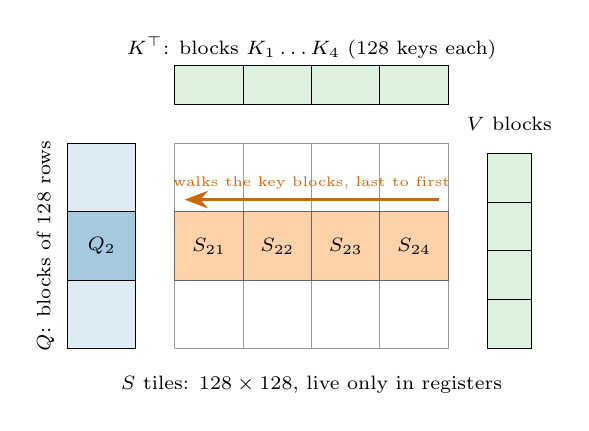
\begin{tikzpicture}[scale=0.62, every node/.style={font=\scriptsize}]
% K^T on top
\foreach \j in {0,...,3} { \draw[fill=okgreen!15] (\j*1.4+2.2,5.0) rectangle ++(1.4,0.8); }
\node at (5.0,6.15) {$K^\top$: blocks $K_1\ldots K_4$ (128 keys each)};
% Q on the left
\foreach \i in {0,...,2} { \draw[fill=validblue!15] (0,\i*1.4) rectangle ++(1.4,1.4); }
\node[rotate=90] at (-0.45,2.1) {$Q$: blocks of 128 rows};
% S grid
\foreach \i in {0,...,2} { \foreach \j in {0,...,3} { \draw[black!40] (\j*1.4+2.2,\i*1.4) rectangle ++(1.4,1.4); } }
\fill[infor!35] (2.2,1.4) rectangle ++(5.6,1.4);
\foreach \j in {0,...,3} { \draw[black!60] (\j*1.4+2.2,1.4) rectangle ++(1.4,1.4); }
\fill[validblue!40] (0,1.4) rectangle ++(1.4,1.4); \draw (0,1.4) rectangle ++(1.4,1.4);
\node at (0.7,2.1) {$Q_2$};
\foreach \j/\n in {0/1,1/2,2/3,3/4} { \node at (\j*1.4+2.9,2.1) {$S_{2\n}$}; }
\draw[-{Stealth}, very thick, infor!80!black] (7.6,3.05) -- (2.4,3.05) node[midway, above, font=\tiny] {walks the key blocks, last to first};
\node[align=center] at (5.0,-0.75) {$S$ tiles: $128\times128$, live only in registers};
% V on the right
\foreach \j in {0,...,3} { \draw[fill=okgreen!15] (8.6,\j*1.0) rectangle ++(0.9,1.0); }
\node[align=center] at (9.05,4.6) {$V$ blocks};
\end{tikzpicture}
\end{column}
\begin{column}{0.43\textwidth}
\small
\begin{itemize}
\item PyTorch 2.6, FP16, $d=32$:\\ {\scriptsize\code{Flash_fwd_kernel_traits<32,128,128,4>}}
  \begin{itemize}\scriptsize
  \item tile $k_M\times k_N = 128\times128$ (queries $\times$ keys)
  \item 4 warps = 128 threads per CTA
  \item grid $(\lceil N/128\rceil,\ \text{batch},\ \text{heads})$
  \end{itemize}
\item CTA $i$ keeps $Q_i$ in \textbf{shared memory}, streams $K_j$, $V_j$ through shared memory, and keeps $S_{ij}$, $P_{ij}$, $\tilde O_i$, $m$, $\ell$ in \textbf{registers}
\item $QK^\top$ and $PV$ run on tensor cores: \code{HMMA.16816.F32} (FP16 in, FP32 accumulate)
\end{itemize}
\end{column}
\end{columns}
\end{frame}

%-----------------------------------------------------------------------------
\begin{frame}[fragile]{The flash kernel, step by step (\code{flash_fwd_kernel.h})}
\begin{columns}[T]
\begin{column}{0.54\textwidth}
\begin{lstlisting}
load Q_i -> sQ           // rows < seqlen_q only
for n_block = last .. first:
  load K_j -> sK, V_j -> sV  // V: OOB rows = 0
  acc_s = Q_i K_j^T      // HMMA, FP32 regs
  mask(acc_s)            // OOB / causal: = -inf
  softmax_rescale_o(acc_s, acc_o)
    // m' = max(m, rowmax)
    // P = 2^(S*s2 - m'*s2), update l
    // acc_o *= 2^((m - m')*s2)
  acc_o += P V_j         // HMMA
lse = normalize_softmax_lse(acc_o) // guard
sO = FP16(acc_o), staged AT THE ADDRESS OF sQ
copy sO -> O,  rows < seqlen_q only
store lse,     rows < seqlen_q only
\end{lstlisting}
\end{column}
\begin{column}{0.44\textwidth}
\small
\begin{itemize}
\item Base 2: $\sigma_2=\sigma\log_2 e$, so $e^{\sigma(x-m)}=2^{x\sigma_2-m\sigma_2}$, one \code{MUFU.EX2}
\item Masking \emph{assigns} $-\infty$; it does not add
\item The output staging reuses the Q buffer: $Q_i$ is no longer needed
\item Stores are \textbf{predicated on the row index}
\end{itemize}
\vspace{1mm}
\begin{block}{The per-row guard (\code{softmax.h:174--177})}\scriptsize
\texttt{sum = row\_sum(mi);}\\
\texttt{lse = (sum == 0.f || sum != sum)}\\
\texttt{\ \ ? (Split ? -INFINITY : INFINITY)}\\
\texttt{\ \ : row\_max * softmax\_scale + \_\_logf(sum);}
\end{block}
\end{column}
\end{columns}
\end{frame}

%-----------------------------------------------------------------------------
\begin{frame}{Split-KV: when there are too few query blocks}
\begin{columns}[c]
\begin{column}{0.55\textwidth}
\centering
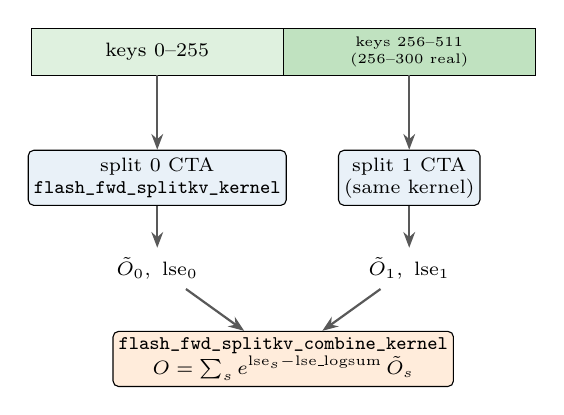
\begin{tikzpicture}[font=\scriptsize]
\draw[fill=okgreen!15] (0,0) rectangle (3.2,0.6); \node at (1.6,0.3) {keys 0--255};
\draw[fill=okgreen!30] (3.2,0) rectangle (6.4,0.6); \node[align=center, font=\tiny] at (4.8,0.3) {keys 256--511\\(256--300 real)};
\node[op, fill=validblue!10] (c0) at (1.6,-1.3) {split 0 CTA\\\code{flash_fwd_splitkv_kernel}};
\node[op, fill=validblue!10] (c1) at (4.8,-1.3) {split 1 CTA\\(same kernel)};
\draw[arr] (1.6,0) -- (c0); \draw[arr] (4.8,0) -- (c1);
\node[font=\scriptsize] (r0) at (1.6,-2.45) {$\tilde O_0,\ \mathrm{lse}_0$};
\node[font=\scriptsize] (r1) at (4.8,-2.45) {$\tilde O_1,\ \mathrm{lse}_1$};
\draw[arr] (c0) -- (r0); \draw[arr] (c1) -- (r1);
\node[op, fill=infor!15] (cb) at (3.2,-3.6) {\code{flash_fwd_splitkv_combine_kernel}\\ $O=\sum_s e^{\mathrm{lse}_s-\mathrm{lse\_logsum}}\,\tilde O_s$};
\draw[arr] (r0) -- (cb); \draw[arr] (r1) -- (cb);
\end{tikzpicture}
\end{column}
\begin{column}{0.43\textwidth}
\small
\begin{itemize}
\item Decode: $N=1$ gives 1 query block per head, too few CTAs for 82 SMs
\item \code{num_splits_heuristic} splits the keys; split kernel tile $64\times256$, so splitting needs $N_k>256$
\item Each split writes a partial output and its own LSE. \textbf{\code{Split=true}}: a zero or \NaN{} row sum gives $\mathrm{lse}_s=-\infty$
\item A split with no key block (causal) writes $-\infty$ directly
\item The combine kernel merges the splits per row, 16 rows per block
\end{itemize}
\end{column}
\end{columns}
\end{frame}

%-----------------------------------------------------------------------------
\begin{frame}[fragile]{The combine kernel and its guard}
\begin{lstlisting}
lse_max = lse_max == -INFINITY ? 0.0f : lse_max;  // In case all local LSEs are -inf
float lse_sum = expf(lse_accum(0) - lse_max);
for (int l = 1; l < kNLsePerThread; ++l) { lse_sum += expf(lse_accum(l) - lse_max); }
lse_sum = Allreduce<kRowsPerLoadTranspose>::run(lse_sum, sum_op);
// For the case where all local lse == -INFINITY, we want to set lse_logsum to INFINITY. Otherwise
// lse_logsum is log(0.0) = -INFINITY and we get NaN when we do lse_accum(l) - lse_logsum.
ElementAccum lse_logsum = (*@\colorbox{infor!25}{(lse\_sum == 0.f || \textbf{lse\_sum != lse\_sum})}@*) ? INFINITY : logf(lse_sum) + lse_max;
\end{lstlisting}
\begin{columns}[T]
\begin{column}{0.5\textwidth}
\small
\begin{itemize}
\item $\mathrm{lse\_logsum}=\log\sum_s e^{\mathrm{lse}_s}$, computed with max subtraction
\item scales $e^{\mathrm{lse}_s-\mathrm{lse\_logsum}}$ weight the partial outputs
\end{itemize}
\end{column}
\begin{column}{0.48\textwidth}
\small
\begin{itemize}
\item \code{lse_sum == 0}: all splits $-\infty$. Writing $+\infty$ makes the scales $e^{-\infty-\infty}=0$, not $e^{-\infty+\infty}=$ \NaN
\item \textbf{\code{lse_sum != lse_sum}}: the comment gives no case. Part 5 shows why
\end{itemize}
\end{column}
\end{columns}
\end{frame}

%=============================================================================
\section{Padding lanes}

\begin{frame}{A decode step in a $128\times128$ tile}
\begin{columns}[c]
\begin{column}{0.52\textwidth}
\centering
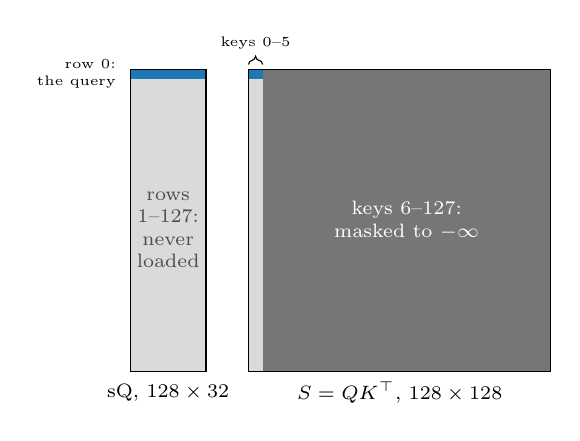
\begin{tikzpicture}[scale=0.03, every node/.style={font=\scriptsize}]
\fill[padgray!35] (0,0) rectangle (32,128);
\fill[validblue] (0,124) rectangle (32,128);
\draw (0,0) rectangle (32,128);
\node at (16,-9) {sQ, $128\times32$};
\node[align=center, text=black!70] at (16,60) {rows\\1--127:\\never\\loaded};
\node[anchor=east, font=\tiny, align=right] at (-2,126) {row 0:\\the query};
\begin{scope}[xshift=50cm]
\fill[padgray!35] (0,0) rectangle (128,128);
\fill[maskdark!70] (6,0) rectangle (128,128);
\fill[validblue] (0,124) rectangle (6,128);
\draw (0,0) rectangle (128,128);
\node at (64,-9) {$S=QK^\top$, $128\times128$};
\node[text=white, align=center] at (67,64) {keys 6--127:\\masked to $-\infty$};
\draw[decorate, decoration={brace, amplitude=3pt}] (0,130) -- (6,130) node[midway, above=2pt, font=\tiny] {keys 0--5};
\end{scope}
\end{tikzpicture}\\[2mm]
\scriptsize\legendbox{validblue} real work: 1 row $\times$ 6 keys \quad \legendbox{padgray!35} padding lanes \quad \legendbox{maskdark!70} masked
\end{column}
\begin{column}{0.46\textwidth}
\small
TinyGPT completes \code{312}; the last forward pass is a decode step per layer:
\begin{itemize}
\item $N=1$ query, $N_k=6$ keys (BOS, 3, 1, 2, and two generated digits)
\item one CTA per head, one $128\times128$ tile
\item \textbf{1 of 128 query rows and 6 of 128 key columns are real}: 24 of 16{,}384 scores per head (0.15\%)
\end{itemize}
\vspace{1mm}
The other 99.85\% are \emph{padding lanes}. The tensor cores compute them anyway: an MMA instruction covers the whole fragment.
\end{column}
\end{columns}
\end{frame}

%-----------------------------------------------------------------------------
\begin{frame}[fragile]{What flash loads, and what it deliberately does not}
\begin{lstlisting}
// We don't need to clear the sQ smem tiles since we'll only write out the valid outputs
copy<Is_even_MN, Is_even_K>(gmem_tiled_copy_QKV, tQgQ, tQsQ, tQcQ, tQpQ, actual_seqlen_q - m_block * kBlockM);
...
// We don't need to clear the sK smem tiles since we'll mask out the scores anyway.
copy<Is_even_MN, Is_even_K>(gmem_tiled_copy_QKV, tKgK, tKsK, tKVcKV, tKVpKV, actual_seqlen_k - n_block * kBlockN);
...
copy<Is_even_MN, Is_even_K, /*Clear_OOB_MN=*/true>(gmem_tiled_copy_QKV, tVgV, tVsV, ...);
\end{lstlisting}
\vspace{1mm}
\begin{center}\scriptsize
\begin{tabular}{l>{\raggedright\arraybackslash}p{3.4cm}>{\raggedright\arraybackslash}p{5.6cm}>{\raggedright\arraybackslash}p{2.6cm}}
\toprule
tile & rows beyond the sequence & why it is safe (claimed) & cost saved \\
\midrule
sQ & \textbf{not loaded, not cleared} & those output rows are never stored & a clear per launch \\
sK & \textbf{not loaded, not cleared} & those scores are masked to $-\infty$ & a clear per key block \\
sV & cleared to 0 & $P=0$ there, but $0\cdot\NaN=\NaN$, so V \emph{must} be clean & --- \\
\bottomrule
\end{tabular}
\end{center}
\vspace{1mm}
\small So the padding rows of sQ and sK hold \textbf{whatever the shared memory last contained}. What is that?
\end{frame}

%-----------------------------------------------------------------------------
\begin{frame}{Scenario: the last launch's \NaN-laden output becomes this launch's Q}
\begin{columns}[c]
\begin{column}{0.58\textwidth}
\centering
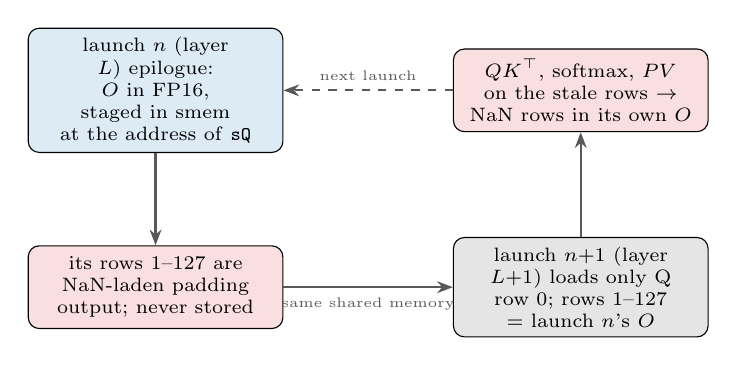
\begin{tikzpicture}[font=\scriptsize, box/.style={draw, rounded corners, text width=3.0cm, minimum height=1.05cm, align=center}]
\node[box, fill=validblue!15] (a) at (0,2.5) {launch $n$ (layer $L$) epilogue:\\$O$ in FP16, staged in smem\\at the address of \code{sQ}};
\node[box, fill=nanred!15] (b) at (0,0) {its rows 1--127 are \NaN{}-laden padding output; never stored};
\node[box, fill=padgray!25] (c) at (5.4,0) {launch $n{+}1$ (layer $L{+}1$) loads only Q row 0; rows 1--127 = launch $n$'s $O$};
\node[box, fill=nanred!15] (d) at (5.4,2.5) {$QK^\top$, softmax, $PV$ on the stale rows $\to$ \NaN{} rows in its own $O$};
\draw[arr] (a) -- (b);
\draw[arr] (b) -- node[below, font=\tiny]{same shared memory} (c);
\draw[arr] (c) -- (d);
\draw[arr, dashed] (d) -- node[above, font=\tiny]{next launch} (a);
\end{tikzpicture}
\end{column}
\begin{column}{0.40\textwidth}
\small Measured, calls 8--11 (the 4 layers of the last decode step), 508 stale Q rows each:
\begin{itemize}
\item \textbf{416} stale Q rows are bit-identical to rows of an earlier call's $O$ tile
\item call 8's 130 \NaN{} $O$ rows $\to$ call 9's stale Q has 3{,}234 \NaN{} values
\item the other stale rows: zero, or from other kernels on the same SM
\item stale K rows: 404 zero, 84 old K rows
\item a second identical run: \textbf{different} stale tiles, \textbf{bitwise-identical} output
\end{itemize}
\end{column}
\end{columns}
\end{frame}

%-----------------------------------------------------------------------------
\begin{frame}{The dumped tiles (call 11 = layer 3, head 0, every element)}
\begin{columns}[c]
\begin{column}{0.64\textwidth}
\centering
\setlength{\tabcolsep}{2pt}
\begin{tabular}{ccccc}
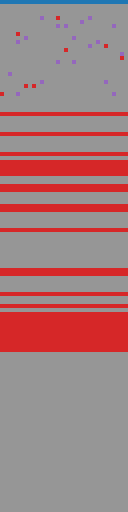
\includegraphics[height=0.30\textheight,interpolate=false]{figs/tile_Q.png} &
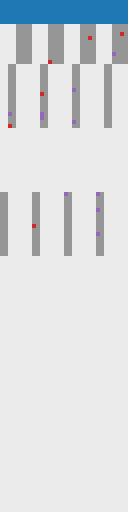
\includegraphics[height=0.30\textheight,interpolate=false]{figs/tile_K.png} &
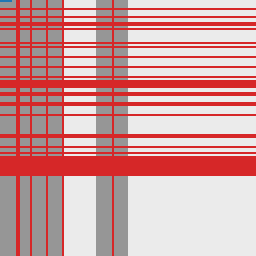
\includegraphics[height=0.30\textheight,interpolate=false]{figs/tile_S_RAW.png} &

\includegraphics[height=0.30\textheight,interpolate=false]{figs/tile_S_MASK.png} &

\includegraphics[height=0.30\textheight,interpolate=false]{figs/tile_P.png}\\
\scriptsize sQ & \scriptsize sK & \scriptsize $S=QK^\top$ & \scriptsize $S$ masked & \scriptsize $P$
\end{tabular}\\[2mm]
\scriptsize
\legendbox{validblue} in sequence \enspace \legendbox{padgray} finite padding \enspace \legendbox{black!8} zero \enspace \legendbox{nanred} \NaN \enspace \legendbox{maskdark} $-\infty$ (mask)
\end{column}
\begin{column}{0.34\textwidth}
\small
\begin{itemize}
\item rows top to bottom = queries; columns = head dim (sQ, sK) or keys
\item the real work: the blue segment at the top left
\item \textcolor{nanred}{\NaN{} rows} of $S$: stale Q rows with \NaN{}
\item \textcolor{nanred}{\NaN{} columns} of $S$: stale K rows with \NaN{}
\item the mask overwrites the columns; \textbf{the rows survive into $P$}
\end{itemize}
\end{column}
\end{columns}
\end{frame}

%=============================================================================
\section{Compute, then discard}

\begin{frame}{How flash computes on the stale lanes (call 11, 4 heads)}
\begin{columns}[T]
\begin{column}{0.50\textwidth}
\scriptsize
\begin{tabular}{@{}lrr@{}}\toprule
region & values & \NaN\\\midrule
Q row 0 (loaded) & 128 & 0\\
\textbf{Q rows 1--127 (stale)} & 16{,}256 & \textbf{3{,}239}\\
K rows 6--127 (stale) & 15{,}616 & 13\\
V rows 6--127 (cleared) & 15{,}616 & 0 (all 0)\\
$S$, real row, keys 0--5 & 24 & 0\\
$S$, real row, padding keys & 488 & 13\\
\textbf{$S$, padding rows} & 65{,}024 & \textbf{18{,}274}\\
$S$ masked, padding rows & 65{,}024 & 798 (+61{,}976 $-\infty$)\\
\textbf{$P$, padding rows} & 65{,}024 & \textbf{798}\\
\textbf{$O$, padding rows} & 16{,}256 & \textbf{4{,}256}\\
$O$, row 0 (the output) & 128 & \textbf{0}\\\bottomrule
\end{tabular}
\end{column}
\begin{column}{0.48\textwidth}
\small Follow one stale row with a \NaN{} in its Q:
\begin{enumerate}
\item $S$ row $=q\cdot K^\top$: \NaN{} in every column
\item mask: columns 6--127 $\to-\infty$; \NaN{} stays in columns 0--5
\item row max ignores \NaN{} (\code{fmaxf}): $m=-\infty$, so \code{max_scaled}$=0$
\item $P=2^{\NaN}$: \NaN{} in 6 columns, 0 elsewhere
\item $\ell=$ \NaN{} $\Rightarrow$ \code{softmax.h}: \code{sum != sum}, $\mathrm{lse}=+\infty$
\item $O$ row $=PV$: \NaN{} in all 32 columns
\end{enumerate}
133 such rows: $133\times6=$ \textbf{798} \NaN{} in $P$, $133\times32=$ \textbf{4{,}256} in $O$
\end{column}
\end{columns}
\end{frame}

%-----------------------------------------------------------------------------
\begin{frame}{Why the results are discarded, and why that is safe}
\centering
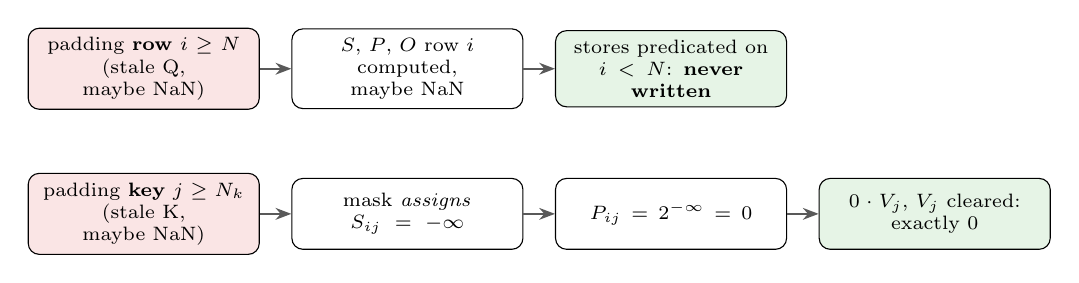
\begin{tikzpicture}[font=\scriptsize, node distance=4mm,
  r/.style={draw, rounded corners, minimum height=9mm, text width=27mm, align=center}]
\node[r, fill=nanred!12] (pr) {padding \textbf{row} $i\ge N$\\(stale Q, maybe \NaN)};
\node[r, right=of pr] (pr2) {$S$, $P$, $O$ row $i$\\computed, maybe \NaN};
\node[r, right=of pr2, fill=okgreen!12] (pr3) {stores predicated on\\$i<N$: \textbf{never written}};
\draw[arr] (pr) -- (pr2); \draw[arr] (pr2) -- (pr3);
\node[r, below=8mm of pr, fill=nanred!12] (pc) {padding \textbf{key} $j\ge N_k$\\(stale K, maybe \NaN)};
\node[r, right=of pc] (pc2) {mask \emph{assigns}\\$S_{ij}=-\infty$};
\node[r, right=of pc2] (pc3) {$P_{ij}=2^{-\infty}=0$};
\node[r, right=of pc3, fill=okgreen!12] (pc4) {$0\cdot V_j$, $V_j$ cleared:\\exactly 0};
\draw[arr] (pc) -- (pc2); \draw[arr] (pc2) -- (pc3); \draw[arr] (pc3) -- (pc4);
\end{tikzpicture}
\vspace{3mm}
\begin{columns}[T]
\begin{column}{0.5\textwidth}
\small
\begin{itemize}
\item \textbf{Rows are independent} (slide 3): a padding row's garbage cannot reach a real row, so it can be computed and dropped
\item \textbf{Keys are mixed into every row}, so padding keys must be neutralized: the mask overwrites the score, and V is cleared so that $0\cdot V=0$
\end{itemize}
\end{column}
\begin{column}{0.48\textwidth}
\small
\begin{itemize}
\item \textbf{Why not clear?} Clearing sQ and sK costs shared-memory stores every launch, for lanes that never matter. Predicated stores are free
\item Also dropped: the padding rows' LSE ($+\infty$ from the guard)
\item The real row's 13 \NaN{} padding-key scores are masked to $-\infty$: harmless
\end{itemize}
\end{column}
\end{columns}
\end{frame}

%-----------------------------------------------------------------------------
\begin{frame}{What this means for a binary-level NaN detector}
\begin{itemize}
\item The \NaN{}s are \textbf{real values in real registers}: \code{HMMA} operands, \code{FADD}/\code{FMUL} in the softmax, \code{MUFU.EX2}
\item A tool that checks instruction operands (nixnan) reports them: \textbf{thousands of \NaN{} sites} in \code{flash_fwd_kernel} while every tensor the model sees is finite
\item Counts vary from run to run and irregularly with sequence length: they depend on what the previous kernel on that SM left in shared memory
\item \code{softmax.h}'s \code{sum != sum} disjunct fires on padding rows (133 of 508 in call 11), never on real rows
\item The same pattern appears in any tiled kernel: cuBLAS/CUTLASS GEMMs, PyTorch's warp softmax (which pads with $-\infty$)
\end{itemize}
\vspace{2mm}
\begin{block}{Lesson}
\textbf{A \NaN{} in a register is not a \NaN{} in the program.} To tell them apart you need the lane's row and column against the sequence bounds, or you check what is stored.
\end{block}
\end{frame}

%=============================================================================
\section{When the guard does not fire}

\begin{frame}{Scenarios A and B: the combine guard on clean and poisoned input}
\begin{columns}[T]
\begin{column}{0.55\textwidth}
\small 301-key prompt, so PyTorch picks 2 KV splits for every call; 12 calls, 4 heads. B adds $+\infty$ to one coordinate of the last prompt embedding.\\[2mm]
\scriptsize
\resizebox{\linewidth}{!}{%
\begin{tabular}{@{}lrr@{}}\toprule
 & A (clean) & B ($+\infty$)\\\midrule
split \code{softmax.h}, real rows: \code{sum != sum} $\to-\infty$ & 0 & \textbf{1{,}144}\\
split \code{softmax.h}, padding rows: \code{sum != sum} & 1{,}588 & 3{,}931\\
combine guard fired, real rows & 0 & \textbf{568}\\
\quad via \code{lse_sum == 0} & 0 & 568\\
\quad via \textbf{\code{lse_sum != lse_sum}} & \textbf{0} & \textbf{0}\\
combine guard, padding rows (16-row block tail), \code{== 0} & 144 & 144\\
output rows with \NaN & 0 & 752\\\bottomrule
\end{tabular}}
\end{column}
\begin{column}{0.43\textwidth}
\small
\begin{itemize}
\item Even with an $\infty$ injected, \textbf{the \NaN{} disjunct never fires}
\item The \NaN{} is removed one level earlier: in the split kernel, \code{softmax.h} maps a \NaN{} row sum to $\mathrm{lse}_s=-\infty$
\item The combine then sees only finite or $-\infty$ LSEs; when all are $-\infty$, $\mathrm{lse\_sum}=0$ exactly
\item The guard cleans the LSE, \textbf{not $O$}: 752 \NaN{} rows vs 568 firings ($0\cdot\NaN$ in $O \mathrel{+}= e^{\ldots}\tilde O_s$)
\end{itemize}
\end{column}
\end{columns}
\end{frame}

%-----------------------------------------------------------------------------
\begin{frame}{Why it cannot fire: the argument in three steps}
\begin{enumerate}
\item \textbf{Combine.} $\mathrm{lse\_sum}=\sum_s e^{\mathrm{lse}_s-L}$, $L=\max_s \mathrm{lse}_s$. It is \NaN{} only if some $\mathrm{lse}_s$ is \NaN{}, or some $\mathrm{lse}_s=+\infty$ ($L=+\infty$, $\infty-\infty$).\\
  Otherwise $\mathrm{lse\_sum}\in\{0\}\cup[1,n_{\text{splits}}]$.
\item \textbf{Split kernel.} $\mathrm{lse}_s=(\ell=0\lor\ell\neq\ell)\ ?\ -\infty : m\sigma+\log\ell$.\\
  So $\mathrm{lse}_s\in\{\NaN,+\infty\}$ needs $\ell=+\infty$ (or $m\sigma=+\infty$ with finite $\ell$).
\item \textbf{Softmax terms.} Each term is $2^{\,\mathrm{fl}(x\sigma_2)-\mathrm{fl}(m\sigma_2)}$, and $x\le m$. For $\sigma>0$:
  \begin{itemize}
  \item $\mathrm{fl}(m\sigma_2)$ finite: every exponent $\le0$, every term in $[0,1]$, the max term is 1, so $\ell\in[1,N_k]$, finite
  \item $\mathrm{fl}(m\sigma_2)=\pm\infty$ (overflow or $m=+\infty$): the max term is $2^{\infty-\infty}=$ \NaN{}, so $\ell=$ \NaN{} $\to$ guard $\to-\infty$
  \item $m=-\infty$ (all masked): \code{max_scaled}$=0$, every term $2^{-\infty}=0$, $\ell=0\to-\infty$
  \end{itemize}
\end{enumerate}
\vspace{1mm}
\begin{block}{Proposition}
For any $\sigma>0$ and \emph{any} FP16 Q, K, V (including $\pm\infty$ and \NaN{}), every $\mathrm{lse}_s\in\mathbb{R}\cup\{-\infty\}$, so \code{lse_sum != lse_sum} is false. TinyGPT ($1/\sqrt{32}$) and BioMistral ($1/\sqrt{128}$) can never take it.
\end{block}
\end{frame}

%-----------------------------------------------------------------------------
\begin{frame}[fragile]{A codegen detail the proof depends on, and huge positive scales}
\begin{columns}[T]
\begin{column}{0.5\textwidth}
\small Source (\code{softmax.h}):
\begin{lstlisting}
// max * log_2(e)) This allows the compiler to use the
// ffma instruction instead of fadd and fmul separately.
tensor(mi, ni) = exp2f(tensor(mi, ni) * scale - max_scaled);
\end{lstlisting}
Compiled split kernel (SASS): \textbf{not fused}
\begin{lstlisting}
FMUL R28, R28, c[0x0][0x238] ;     // x * scale
...
FADD R154, -R47, R154 ;            // - max_scaled
FSETP.GEU.AND P1, PT, R160, -126, PT ;
MUFU.EX2 R160, R160 ;
\end{lstlisting}
\small Two roundings, so overflow of $m\sigma_2$ yields $\infty-\infty$ = \NaN{}, which the guard catches.
\end{column}
\begin{column}{0.48\textwidth}
\small Raw flash call, $N_k=301$, 2 splits, head 0 (our build and PyTorch's agree, \NaN-aware):\\[1mm]
\scriptsize
\begin{tabular}{@{}llll@{}}\toprule
$\sigma$ & split 0: $m$, $\ell$, lse & combine & fires\\\midrule
$1/\sqrt{32}$ & 15.2, 33.1, 6.19 & 1.23 & 0/4\\
$10^{30}$ & $-37.1$, 256, $-3.7\!\cdot\!10^{31}$ & 1 & 0/4\\
$10^{37}$ & $-37.1$, \textbf{\NaN}, $-\infty$ & 1 & 0/4\\\bottomrule
\end{tabular}\\[2mm]
\small At $\sigma=10^{37}$, $m\sigma_2$ overflows; unfused code gives $\ell=$ \NaN{} and \code{softmax.h} catches it.\\[1mm]
A \emph{fused} \code{FFMA} would give $\ell=+\infty$ and open the door, but only for $\sigma>1.7\cdot10^{27}$ with FP16 inputs.
\end{column}
\end{columns}
\end{frame}

%=============================================================================
\section{Making it fire}

\begin{frame}{A negative softmax scale breaks the premise}
\begin{columns}[c]
\begin{column}{0.47\textwidth}
\small
\begin{itemize}
\item The proof used $x\le m \Rightarrow x\sigma_2\le m\sigma_2$. With $\sigma<0$ the order flips: the exponent is $(m-x)\,|\sigma_2|\ \ge 0$
\item A \textbf{masked} score $x=-\infty$: $(-\infty)\cdot\sigma_2=+\infty$, so the term is $2^{+\infty}=+\infty$
\item Large score spreads overflow too: $(m-x)|\sigma_2|>128$
\item $\ell=+\infty$ is neither 0 nor \NaN{}: \code{softmax.h} passes it, $\mathrm{lse}_s=m\sigma+\log\infty=+\infty$
\item \code{F.scaled_dot_product_attention(..., scale=-0.1)} is accepted: neither SDPA nor \code{mha_fwd} checks the sign
\end{itemize}
\end{column}
\begin{column}{0.51\textwidth}
\centering
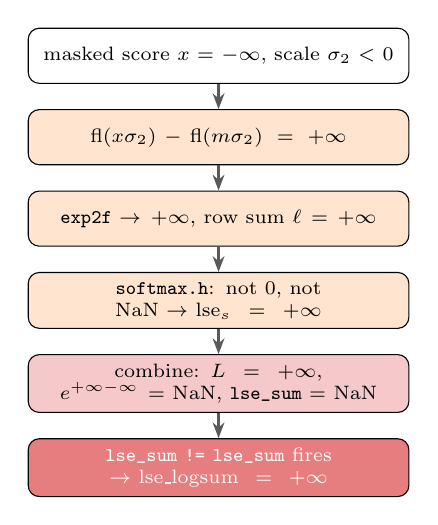
\begin{tikzpicture}[font=\scriptsize, node distance=3.2mm,
  c/.style={draw, rounded corners, minimum height=7mm, text width=46mm, align=center, fill=white}]
\node[c] (a) {masked score $x=-\infty$, scale $\sigma_2<0$};
\node[c, below=of a, fill=infor!20] (b) {$\mathrm{fl}(x\sigma_2)-\mathrm{fl}(m\sigma_2)=+\infty$};
\node[c, below=of b, fill=infor!20] (c) {\code{exp2f} $\to+\infty$, row sum $\ell=+\infty$};
\node[c, below=of c, fill=infor!20] (d) {\code{softmax.h}: not 0, not \NaN{} $\to$ $\mathrm{lse}_s=+\infty$};
\node[c, below=of d, fill=nanred!25] (e) {combine: $L=+\infty$, $e^{+\infty-\infty}=$ \NaN{}, \code{lse_sum} = \NaN};
\node[c, below=of e, fill=nanred!60, text=white] (f) {\textbf{\code{lse_sum != lse_sum}} fires $\to$ $\mathrm{lse\_logsum}=+\infty$};
\draw[arr] (a)--(b); \draw[arr] (b)--(c); \draw[arr] (c)--(d); \draw[arr] (d)--(e); \draw[arr] (e)--(f);
\end{tikzpicture}
\end{column}
\end{columns}
\end{frame}

%-----------------------------------------------------------------------------
\begin{frame}{It fires: one raw flash call (\code{trigger_nan_guard.py})}
\begin{columns}[T]
\begin{column}{0.58\textwidth}
\scriptsize Decode-shaped call: $N=1$, $N_k=301$, 2 splits, 4 heads, random FP16 Q, K, V. Head 0:\\[1mm]
\resizebox{\linewidth}{!}{%
\begin{tabular}{@{}lllll@{}}\toprule
$\sigma$ & split 0: $m$, $\ell$, lse & split 1: $m$, $\ell$, lse & \code{lse_sum} & disjunct\\\midrule
$1/\sqrt{32}$ & 15.23, 33.1, 6.19 & 17.08, 5.52, 4.73 & 1.23 & none, 0/4\\
$10^{37}$ & $-37.1$, \NaN, $-\infty$ & 17.08, 1, $1.7\!\cdot\!10^{38}$ & 1 & none, 0/4\\
$-0.1$ & 15.23, 1435, 5.75 & 17.08, \textbf{$+\infty$}, \textbf{$+\infty$} & \textbf{\NaN} & \textbf{\code{!=}, 4/4}\\
$-1$ & 15.23, $1.9\!\cdot\!10^{16}$, 22.3 & 17.08, $+\infty$, $+\infty$ & \NaN & \code{!=}, 4/4\\
$-10$ & 15.23, $+\infty$, $+\infty$ & 17.08, $+\infty$, $+\infty$ & \NaN & \code{!=}, 4/4\\\bottomrule
\end{tabular}}
\end{column}
\begin{column}{0.40\textwidth}
\small
\begin{itemize}
\item At $\sigma=-0.1$, split 0 is still finite (all 256 keys real, spread $<128/|\sigma_2|$)
\item Split 1 covers keys 256--511, of which 301--511 are beyond the sequence: \textbf{211 masked columns}, each $2^{+\infty}$
\item So the trigger is the \textbf{mask on the padding keys}, the same lanes as part 3
\item Every case matches PyTorch's own kernel
\end{itemize}
\end{column}
\end{columns}
\end{frame}

%-----------------------------------------------------------------------------
\begin{frame}{It fires inside TinyGPT: \code{dump_lse.py --input A --scale -0.1}}
\begin{columns}[T]
\begin{column}{0.55\textwidth}
\scriptsize Clean input A, every attention call with $\sigma=-0.1$:\\[1mm]
\resizebox{\linewidth}{!}{%
\begin{tabular}{@{}lrrr@{}}\toprule
calls & fired & via \code{== 0} & via \textbf{\code{!=}}\\\midrule
0: layer 0 prefill (301 rows/head) & 1{,}200 & 0 & \textbf{1{,}200}\\
1--3: layers 1--3 prefill & 3{,}612 & 3{,}612 & 0\\
4, 8: layer 0 decode & 8 & 0 & \textbf{8}\\
5--7, 9--11: layers 1--3 decode & 24 & 24 & 0\\\midrule
total & 4{,}844 & 3{,}636 & \textbf{1{,}208}\\
default scale & 0 & 0 & 0\\\bottomrule
\end{tabular}}\\[2mm]
\small Completion: \code{312452} becomes \code{...312000}.
\end{column}
\begin{column}{0.43\textwidth}
\small
\begin{itemize}
\item \textbf{Layer 0}: clean inputs; the causal and padding masks supply the $-\infty$ scores $\Rightarrow$ $\ell=+\infty$, $\mathrm{lse}_s=+\infty$, \code{lse_sum != lse_sum}
\item Only row 255 of each head escapes: it sees all of split 0 unmasked, and split 1 has no key block for it
\item \textbf{Layers 1--3}: inputs already \NaN{} from layer 0, so \code{softmax.h} maps every split to $-\infty$, and the guard fires via \code{lse_sum == 0}, as in scenario B
\end{itemize}
\end{column}
\end{columns}
\end{frame}

%-----------------------------------------------------------------------------
\begin{frame}{What a negative scale would mean in practice}
\begin{itemize}
\item $\mathrm{softmax}(-|\sigma|\,QK^\top)$ attends most to the keys \emph{least} similar to the query: ``anti-attention''. No standard model does this; every trained transformer uses $\sigma=1/\sqrt d>0$
\item Realistic ways to get there: a sign error, or a user-supplied \code{scale=} computed wrongly. The API accepts it silently
\item It is an \textbf{engineered trigger}: the cheapest input that reaches the disjunct, not a scenario BioMistral or TinyGPT can hit in normal use
\item Even when the guard fires, it only fixes the LSE: the outputs of the affected rows are non-finite (1{,}204 rows in layer 0) and the completion degrades
\end{itemize}
\vspace{2mm}
\begin{block}{So what is \code{lse_sum != lse_sum} for?}
Defensive code. With unfused codegen and $\sigma>0$ it is dead. It becomes live with $\sigma<0$, or with a fused-\code{FFMA} build and an absurdly large scale (or BF16 inputs and $\sigma>0.69$).
\end{block}
\end{frame}

%-----------------------------------------------------------------------------
\begin{frame}{Summary}
\begin{enumerate}
\item \textbf{Flash attention} = tiled, fused attention with an online softmax: no $N\times N$ matrix ever reaches memory; per row it keeps $m$, $\ell$, $\tilde O$ and emits $O$ and $\mathrm{lse}=m\sigma+\log\ell$
\item \textbf{Fixed tiles create padding lanes.} A decode step uses 24 of 16{,}384 scores per head
\item \textbf{Unloaded rows hold stale shared memory}, typically the previous launch's \NaN-laden output tile, because $O$ is staged at the Q buffer's address
\item \textbf{Flash computes on them and discards them}: padding rows are never stored (rows are independent); padding keys are overwritten with $-\infty$ and V is cleared ($0\cdot V=0$)
\item \textbf{\code{lse_sum != lse_sum} never fires for $\sigma>0$}, for any input: \code{softmax.h} turns every \NaN{} row sum into $-\infty$ first, and $\ell$ cannot reach $+\infty$
\item \textbf{A negative scale makes it fire}: masked scores become $2^{+\infty}$, $\mathrm{lse}_s=+\infty$, $\infty-\infty$ in the combine. 1{,}208 firings in TinyGPT
\end{enumerate}
\vspace{1mm}
\scriptsize Code and traces: \code{flash-attn-expt/PyTorch_Instrumentation/}. Full report: \code{flash-attn-expt/latex/report.pdf}.
\end{frame}

\end{document}
